\section{Auswertung}
\label{sec:Auswertung}



\subsection{Stabilitätsbedingung}
\label{subsec:Stabil}
Für die beiden Resonatorspiegel werden zwei Spiegel mit einem
Krümmungsradius von $r_{1,2}=\SI{1.4}{\meter}$ verwendet.
Aus Gleichung \eqref{eqn:stabil_params} ergeben sich die beiden
Resonatorparameter in Abhängigkeit der Resonatorlänge $L$.
Laut Stabilitätsbedingung ist der Laser stabil,
wenn $g_1\cdot g_2$ zwischen null und eins liegt.
Die Abbildung \ref{fig:oberaffengeilerplot} enthält $g_1 \cdot g_2$
in Abhängigkeit von der Resonatorlänge $L$.
Desweitern enthält die Abbildung \ref{fig:oberaffengeilerplot}
die Messwerte
für die maximale durch Justage
erreichte Laserleistung $P$
bei einer bestimmten Resonatorlänge
aus der Tabelle \ref{tab:stabil}
und den zugehörigen Parameter $g_1 \cdot g_2$.

\begin{table}
  \centering
  \caption{Unterschiedliche Resonatorlänge $L$ und der zugehörige Stabilitätsparameter $g_1 \cdot g_2$
  sowie die maximal erreichte Laserleistung $P$ bei entsprechender Resonatorlänge.}
  \label{tab:stabil}
  \begin{tabular}{ccc}
\toprule
$L/ \si{\meter}$ & $g_1 \cdot g_2$ & $ P/ \si{\milli\watt}$\\
\midrule
0.53	&	0.3862	&	4.20   \\
0.69	&	0.2572	&	4.56   \\
0.83	&	0.1658	&	4.81   \\
0.98	&	0.0900	&	4.63   \\
1.13	&	0.0372	&	4.13   \\
1.28	&	0.0073	&	3.38   \\
1.43	&	0.0005	&	4.39   \\
1.58	&	0.0165	&	2.52   \\
1.73	&	0.0556	&	2.42   \\
\bottomrule
  \end{tabular}
\end{table}


\begin{figure}
  \centering
  \includegraphics[width=0.9\textwidth]{build/g1g2_Leistung.pdf}
  \caption{Maximal gemessene
  Laserleistung $P$ und
  Stabilitätsparameter $g_1\cdot g_2$ aufgetragen gegen
   die Resonatorlänge $L$, sowie
   die Stabilitätsgrenzen in schwarz.
  }
  \label{fig:oberaffengeilerplot}
\end{figure}



\subsection{Moden}
\label{subsec:tem}
\paragraph{longitudinale Moden}
Die Frequenz der longitudialen Moden $q$
ergibt sich aus der Resonazbedingung
\begin{align}
  \label{eqn:longi_mode}
  \nu=\frac{qc}{2L}
\end{align}
aus der Resonatorlänge $L$ und der Lichtgeschwindigkeit $c$.
Aus dem Frequenzunterschied $\Delta \nu$ zweier benachbarter longitudialer Moden
ergibt sich aus Gleichung \ref{eqn:longi_mode} der Zusammenhang
\begin{align}
  c = 2L\Delta \nu \, ,  \label{eqn:Lichtgeschwindigkeit}
\end{align}
mit dem die Lichtgeschwindigkeit aus bekannter Resonatorlänge und Frequenzspektrum
berechnet werden kann.
In der Abbildung \ref{fig:L1_freq} ist ein Frequenzspekturm für ein Laser mit einer Resonatorlänge $L=\SI{73.5}{\centi\meter}$
dargestellt. Aus diesem werden die Frequenzen $\nu$ abgelesen
 und die Frequenzdifferenzen $\Delta \nu $ bestimmt und die Lichtgeschwindigkeit $c$ nach Gleichung \ref{eqn:Lichtgeschwindigkeit}
berechnet.
Die Tabelle \ref{tab:freq_L1} enthält die entsprechenden Ergebnisse.
Zusätzlich wird eine weitere Resonatorlänge $L = \SI{83.5}{\centi\meter}$  untersucht
(vergleiche Abbildung \ref{fig:L2_freq} und Tabelle \ref{tab:L2_freq}).

\begin{figure}
\centering
  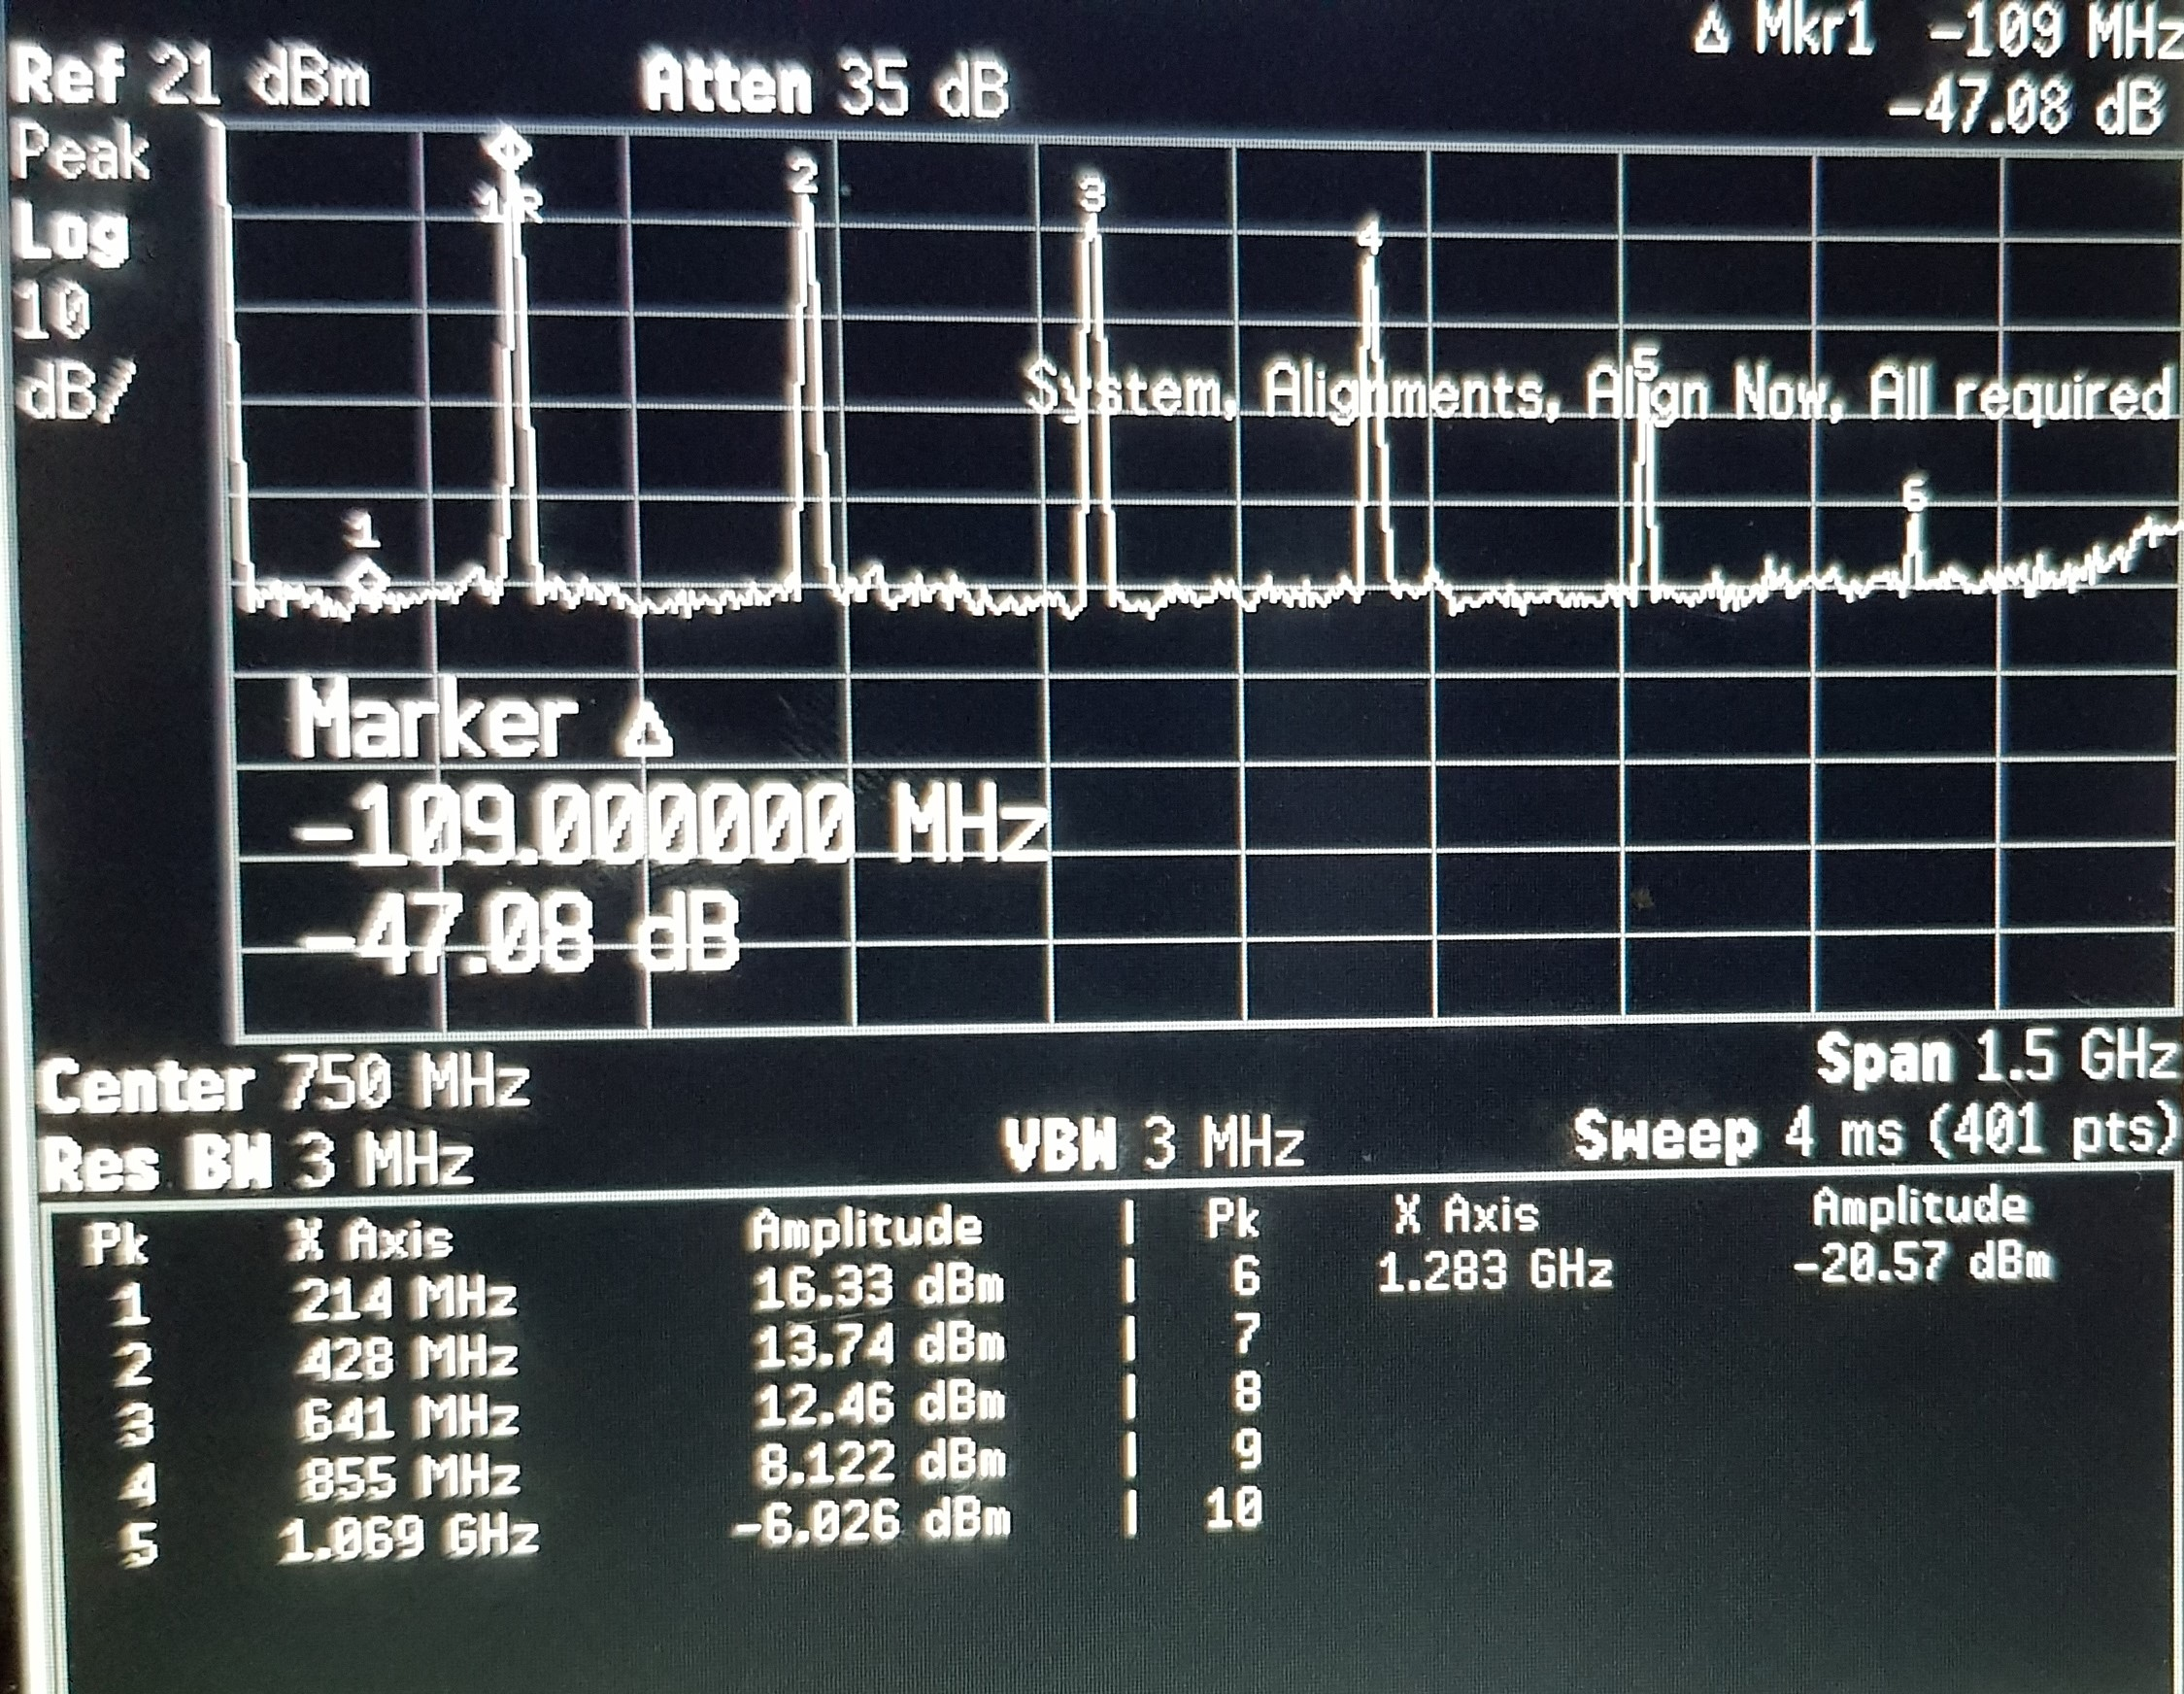
\includegraphics[width=0.7\textwidth]{pictures/freq_1.jpg}
  \caption{Frequenzspektrum bei einer Resonatorlänge von $L=\SI{73.5}{\centi\meter}$.}
  \label{fig:L1_freq}
\end{figure}

\begin{table}
  \centering
\caption{Frequenzen $\nu$ bei einer Resonatorlänge von $L=\SI{73.5}{\centi\meter}$ und die entsprechenden berechneten Größen die Frequenzdifferenzen $\Delta \nu$ und die Lichtgeschwindigkeit $c$.  }
\label{tab:freq_L1}
\begin{tabular}{c c c }
   \toprule
   $\nu /\si{\mega\hertz}$ & $\Delta \nu / \si{\mega\hertz}$ & $c / \SI{e8}{\meter\per\second}$\\
\midrule
214	  \pm	5 	&	 214	\pm	7	&	3.15	\pm	0.10   \\
428	  \pm	5 	&	 213	\pm	7	&	3.13	\pm	0.10   \\
641 	\pm	5	  &  214	\pm	7	&	3.15	\pm	0.10   \\
855 	\pm	5 	&	 214	\pm	7	&	3.15	\pm	0.10   \\
1069	\pm	5 	&	 214	\pm	7	&	3.15	\pm	0.10   \\
1283	\pm	5	  &	 & \\
\bottomrule
\end{tabular}
\end{table}


\begin{figure}
  \centering
  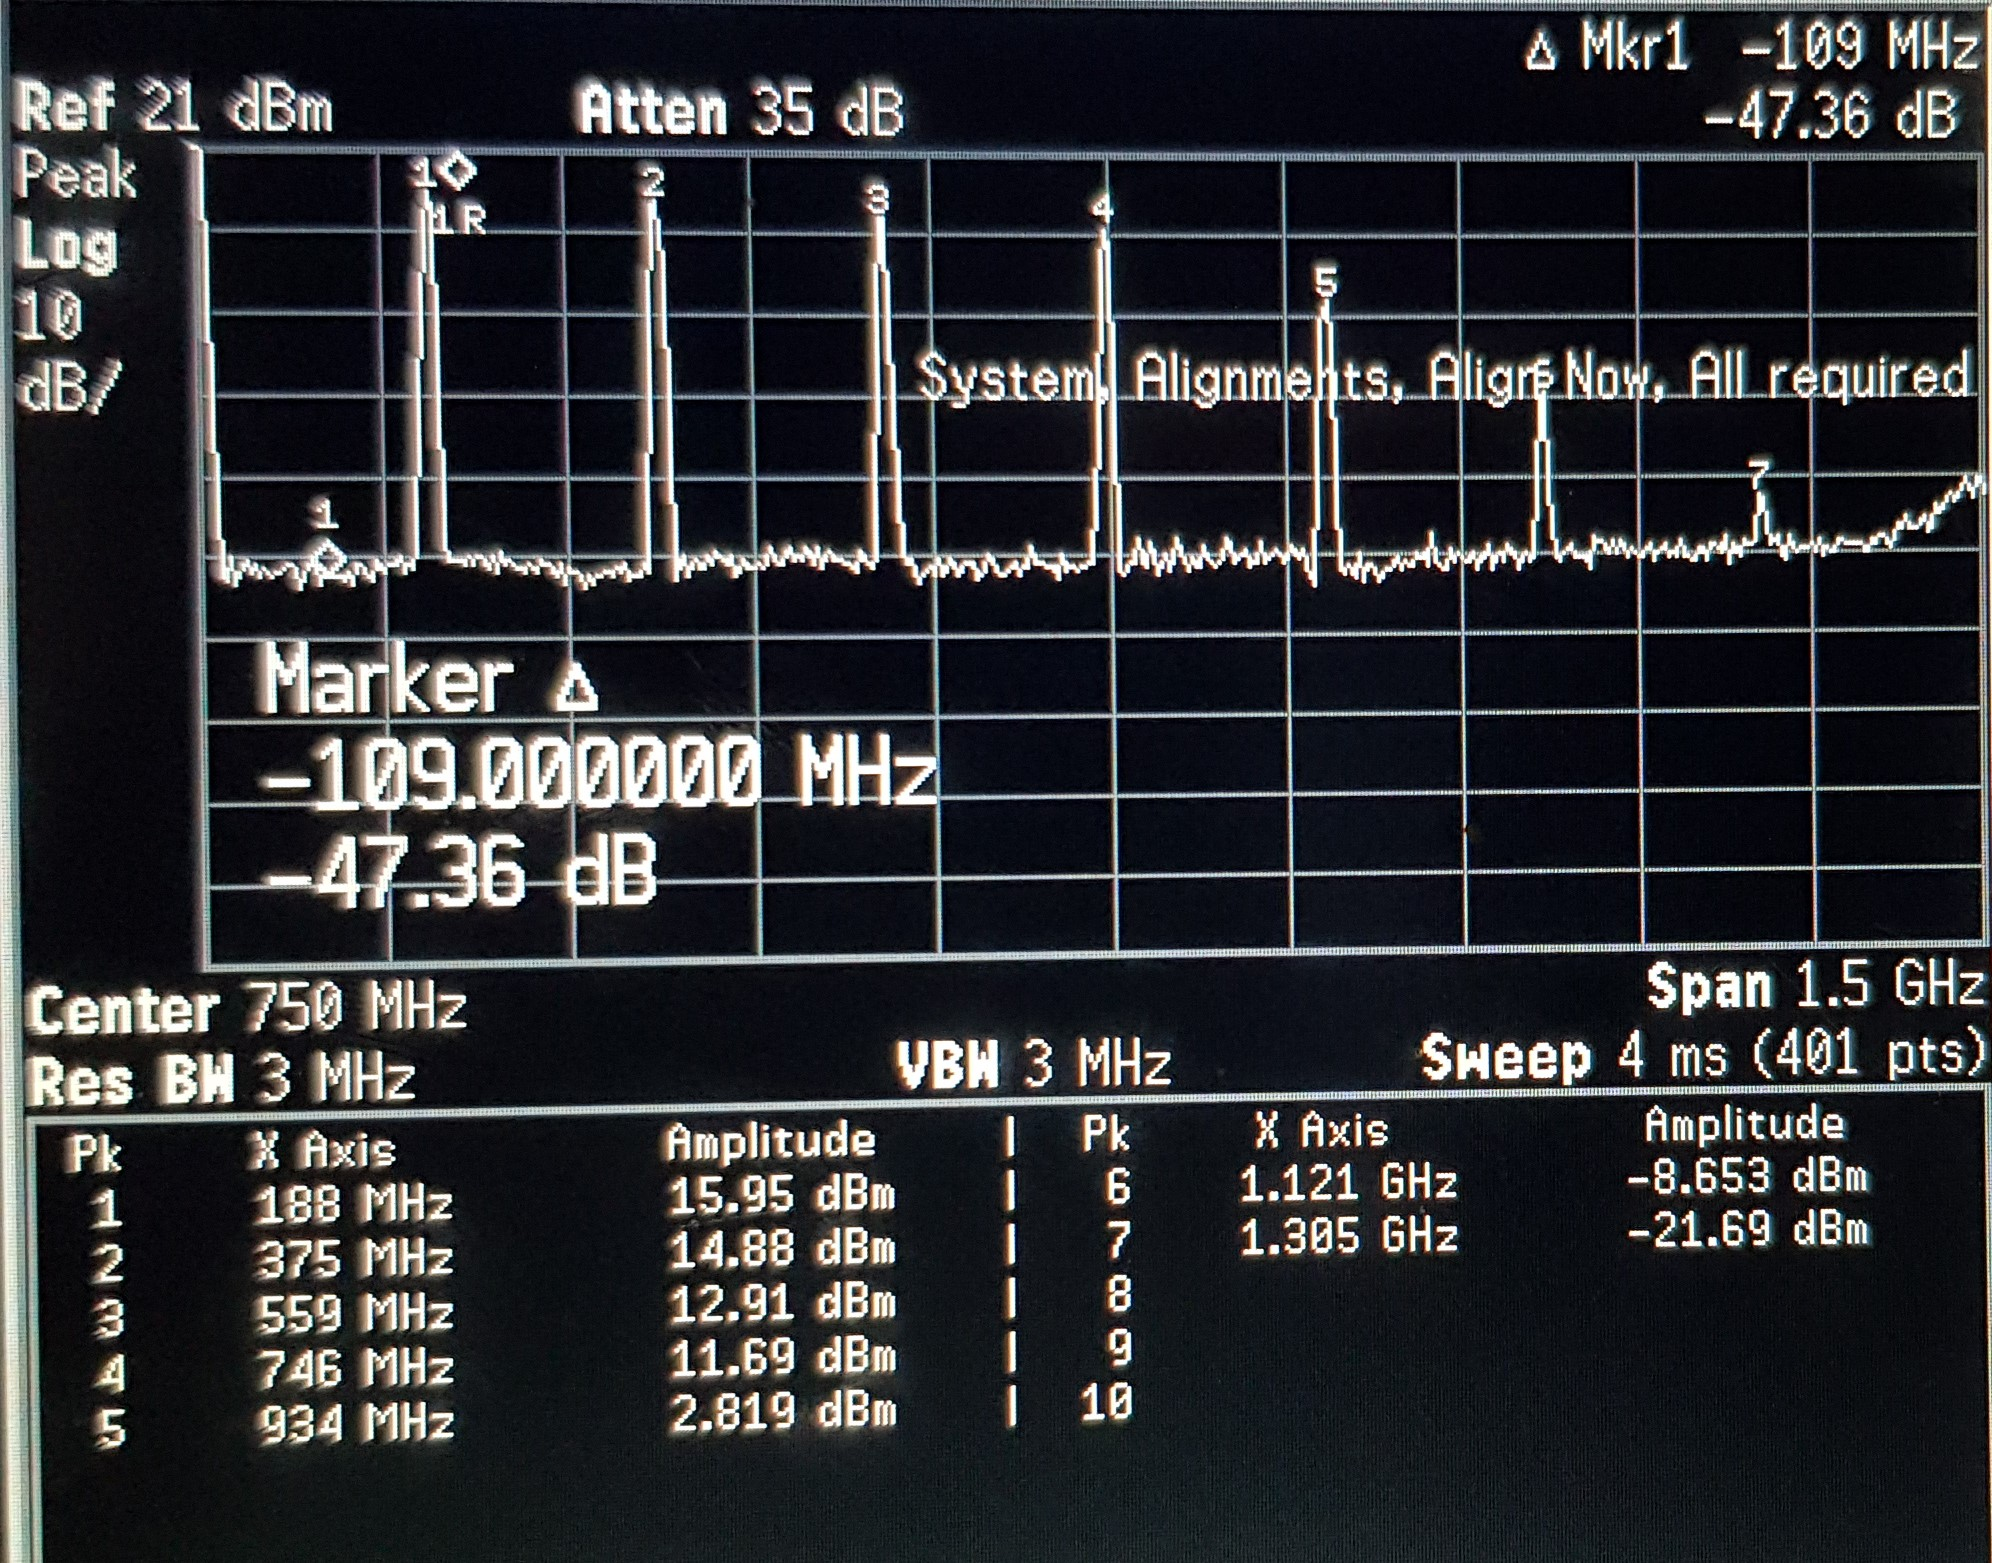
\includegraphics[width=0.7\textwidth]{pictures/freq_2.jpg}
  \caption{Frequenzspektrum bei einer Resonatorlänge von $L = \SI{83.5}{\centi\meter}$.}
  \label{fig:L2_freq}
\end{figure}

\begin{table}
  \centering
\caption{Frequenzen $\nu$ bei einer Resonatorlänge von $L = \SI{83.5}{\centi\meter}$ und die entsprechenden berechneten Größen die Frequenzdifferenzen $\Delta \nu$ und die Lichtgeschwindigkeit $c$.  }
\label{tab:L2_freq}
\begin{tabular}{c c c }
   \toprule
   $\nu /\si{\mega\hertz}$ & $\Delta \nu / \si{\mega\hertz}$ & $c / \SI{e8}{\meter\per\second}$\\
\midrule
	188	 \pm 5  & 187	\pm	7	&	3.12	\pm	0.12   \\
	375	 \pm 5  & 184	\pm	7	&	3.07	\pm	0.12   \\
	559	 \pm 5  & 187	\pm	7	&	3.12	\pm	0.12   \\
	746	 \pm 5  & 188	\pm	7	&	3.14	\pm	0.12   \\
	934	 \pm 5  & 187	\pm	7	&	3.12	\pm	0.12   \\
	1121 \pm 5  & 184	\pm	7	&	3.07	\pm	0.12   \\
  1305 \pm 5\\
\bottomrule
\end{tabular}
\end{table}



\paragraph{transversale Moden}
Weiterhin werden zwei transversale Moden des Lasers untersucht.
Zum einen die \textbf{$\text{TEM}_{00}$},
deren Intensiätsmaximum in der Mitte des Strahls lokalisiert ist(siehe Abbildung \ref{fig:mode00}).
An die aufgenommenen Messwerte wird ein Gaußfit gemäß Gleichung \ref{eqn:TEM00} vorgenommen.
In Abbildung \ref{fig:mode00} ist der entsprechende Graph neben den Messwerten dargstellt.
Es ergeben sich die Fitparameter
\begin{align*}
  I_0 &=\SI{62.3(9)}{\nano\ampere} \\
  \omega &=\SI{13.8(2)}{\milli\meter} \\
  d_0 &=\SI{12.9(1)}{\milli\meter} \, .
\end{align*}
\begin{figure}
  \centering
  \includegraphics{build/mode00.pdf}
  \caption{Gemessene Intensitätsverteilung der \textbf{$\text{TEM}_{00}$}-Mode und Gaußfit an die Messwerte.}
  \label{fig:mode00}
\end{figure}

Zum anderen wird die \textbf{$\text{TEM}_{01}$} untersucht, deren Intensitätsmaxima durch
zwei gleich weit vom Strahlzentrum entfernte Gaußpeaks gegeben sind.
An die aufgenommenen Messwerte wird ein Gaußfit gemäß Gleichung \ref{eqn:TEM01} vorgenommen.
In Abbildung \ref{fig:mode01} ist der entsprechende Graph neben den Messwerten dargstellt.
\begin{align}
  I_{(0,1)}(d) = I_{0} \left( d - d_{0} \right)^{2}
  \exp\left( -2 \left( \frac{d - d_{0}}{\omega}\right)^2 \right)\label{eqn:TEM01}
\end{align}
Es werden die Fitparameter
 \begin{align*}
   I_{0} &= \SI{64.1(147)}{\nano\ampere\per\milli\meter\squared}\\ \omega &=\SI{6.5(5)}{\milli\meter}\\    d_{0} &= \SI{-3.9(4)}{\milli\meter}
 \end{align*}
% I_01,I_02,w1,w2,d_01,d_02
gefunden.
\begin{figure}
  \centering
  \includegraphics{build/mode01.pdf}
  \caption{Gemessene Intensitätsverteilung der \textbf{$\text{TEM}_{01}$}-Mode und Gaußfit an die Messwerte.}
  \label{fig:mode01}
\end{figure}



\subsection{Polarisation}
\label{subsec:Polarisation}
Die Messwerte zur Bestimmung der Polarisation des Lasers sind in Tabelle \ref{tab:polarisation} aufgelistet.
In Abbildung \ref{fig:polarisation} wird die Intensität $I$(gemessen wird ein elektrischer Strom in $\si{\nano\ampere}$)
in Abhängigkeit von dem Polarisationswinkel $\phi$
aufgetragen und die Funktion
\begin{align}
I(\phi)=I_0 \cos^2\left(\phi-\phi_0\right)
\end{align}
an die Messwerte gefittet.
Für die Funktion ergeben sich die Parameter
\begin{align}
I_0  & = \SI{142.4(6)}{\nano\ampere},\\
\phi_{0} & = \SI{68.3(2)}{\degree}.
\end{align}

\begin{table}
  \centering
  \caption{Messwerte der Intensität in Abhängigkeit von dem Winkel des Polarisationsfilters.}
  \label{tab:polarisation}
  \begin{tabular}{c c | c c}
\toprule
    $\phi / \si{\degree}$ & $I/\si{\nano\ampere}$ & $\phi / \si{\degree}$ & $I/\si{\nano\ampere}$\\
\midrule
0	&	24.8   & 190	&	29.2 \\
10	&	51.2 &  200	&	38.0  \\
20	&	83.3 &  210	&	64.5  \\
30	&	119.8&  220	&	71.0   \\
40	&	144.9&  230	&	97.9   \\
50	&	144.1&  240	&	130.1  \\
60	&	111.7&  250	&	112.2  \\
70	&	201.3&  260	&	125.6  \\
80	&	209.4& 270	&	96.9    \\
90	&	130.1& 280	&	76.0    \\
100	&	101.7& 290	&	88.6    \\
110	&	74.8 & 300	&	51.0   \\
120	&	45.3 & 310	&	38.5   \\
130	&	26.4 & 320	&	18.4   \\
140	&	12.4 & 330	&	4.4    \\
150	&	2.8  & 340	&	0.5   \\
160	&	0.5  & 350	&	4.8   \\
170	&	2.5  & 360	&	26.1  \\
180	&	11.7 &  &  \\
\bottomrule
\end{tabular}
\end{table}


\begin{figure}
  \centering
  \includegraphics{build/polarisation.pdf}
  \caption{Intensität in Abhängigkeit des Polarisationswinkel.}
  \label{fig:polarisation}
\end{figure}




\subsection{Wellenlängenbestimmung}
\label{subsec:wellenlaenge}

Die Wellenlänge der charakteristischen roten Linie des He-Ne-Lasers, wird mit Hilfe
von zwei optischen Gittern ($g_{1} = \SI{80}{\per\centi\meter} \ g_{2} = \SI{100}{\per\centi\meter}$) bestimmt.
Es wird jeweils ein Wert zu jedem Maximum bestimmt. Aus dem Mittel der Werte der einzelnen Maxima
wird für jedes Gitter eine Wellenlänge berechnet.
In Tabelle \ref{tab:wellenlaenge} sind jeweils die Werte für Schirmabstand $L$ und Abstände der Maxima
zum Maximum $0.$-Ordnung $d_{\text{i}}$ zusammen mit den bestimmten Wellenlängen angegeben.\\
Es ergibt sich eine mittlere Wellenlänge von
\begin{align*}
  \lambda_{1} &= \SI{6.53(2) e-7}{\meter}\\
  \lambda_{2} &= \SI{6.58(1) e-7}{\meter} \, .
\end{align*}


\begin{table}
\centering
  \caption{Mit zwei optischen Gittern bestimmte Wellenlängen mit jeweiligen relevanten Größen.}
  \label{tab:wellenlaenge}
\begin{tabular}{c|c c || c c}
  & \multicolumn{2}{c}{$g_{1} = \SI{80}{\per\centi\meter}$} & \multicolumn{2}{c}{$g_{2} = \SI{100}{\per\centi\meter}$} \\
\toprule
Ordnung $i$ &    $d_i / \si{\centi\meter}$  & $\lambda / \si{\nano\meter}$ &    $d_i / \si{\centi\meter}$  & $\lambda / \si{\nano\meter}$ \\
\midrule
1 & \phantom{0}7.2 \pm	\, 0.1	&	637.4	\pm	\,8.8	&	\phantom{0}9.2  	\pm	\, 0.1	&	650.0	\pm	\,7.0   \\
2 & 14.5	         \pm	\, 0.1	&	634.9	\pm	\,4.3	&	18.5	            \pm	\, 0.1	&	645.9	\pm	\,3.4   \\
3 & 21.8	         \pm	\, 0.1	&	630.8	\pm	\,2.8	&	27.8	            \pm	\, 0.1	&	639.3	\pm	\,2.2   \\
4 & 29.2	         \pm	\, 0.1	&	630.5	\pm	\,2.1	&	43.0	            \pm	\, 0.1	&	724.6	\pm	\,1.5   \\
5 & 41.2	         \pm	\, 0.1	&	697.4	\pm	\,1.6	&	48.2	            \pm	\, 0.1	&	643.4	\pm	\,1.2   \\
6 & 49.5	         \pm	\, 0.1	&	685.8	\pm	\,1.2	&	59.5	            \pm	\, 0.1	&	644.1	\pm	\,0.9   \\
\bottomrule
\end{tabular}
\end{table}
